\documentclass[]{ccs-thesis}
% options:
% [germanthesis] - Thesis is written in German
% [plainunnumbered] - Don't print numbers on plain pages
% [earlydraft] - Settings for quick draft printouts
% [watermark] - Print current time/date at bottom of each page
% [phdthesis] - switch to PhD thesis style
% [twoside] - double sided
% [cutmargins] - text body fills complete page


% Author name. Separate multiple authors with commas.
\author{Gaurav Kumar Singh}
\birthday{10. November 1989}
\birthplace{Danapur, India}

% Title of your thesis.
\title{Clustering in Vehicular Networks}

% Choose one of the following lines. Feel free to change the word "Informatik" to match your degree program.
%\thesistype{Masterarbeit im Fach Informatik}\thesiscite{Master's Thesis~(Masterarbeit)}
%\thesistype{Bachelorarbeit im Fach Informatik}\thesiscite{Bachelor Thesis~(Bachelorarbeit)}
\thesistype{Seminararbeit im Fach Informatik}\thesiscite{Seminar Thesis~(Seminararbeit)}

% List of advisors, separated by commas.
\advisors{Jun.-Prof. Dr.-Ing. Christoph Sommer, Prof. Dr.-Ing. habil. Falko Dressler}

% List of referees, separated by commas.
\referees{Jun.-Prof. Dr.-Ing. Christoph Sommer, Prof. Dr.-Ing. habil. Falko Dressler}


% Define abbreviations used in the thesis here.
\acrodef{WSN}{Wireless Sensor Network}
\acrodef{WANET}{Wireless Ad Hoc Network}
\acrodef{MANET}{Mobile Ad Hoc Network}
\acrodef{VANET}{Vehicular Ad Hoc Network}
\acrodef{CH}{Cluster Head}
\acrodef{CM}{Cluster Member}
\acrodef{CHP}{Cluster Head Pending}
\acrodef{RSU}{Road Side Unit}
\acrodef{GPS}{Global Positioning System}
\acrodef{VEINS}{Vehicles in Network Simulation}
\acrodef{V2V}{Vehicle-to-Vehicle}
\acrodef{V2I}{Vehicle-to-Infrastructure}

\begin{document}

\pagenumbering{roman}

\maketitle

\chapter*{Abstract}
\addcontentsline{toc}{chapter}{Abstract}
\begin{otherlanguage*}{american}

    This thesis captures an overview of ideas, techniques, results and future possibilities of clustering in vehicular networks.
    Clustering is a technique to group nodes based on a selected criterion which defines certain level of similarities among the nodes.
    Grouping the nodes together in such a way helps to define or design a set of functionalities applicable only to the
    group and can be applied to the smaller sub-set. In a \ac{VANET} environment, clustering presents possibilities
    to group vehicles based on a parameter of interest and help to reduce the network traffic, achieve better network throughput and
    effective information dissemination.

    In this thesis, I try to present some of the parameter and methodologies used for clustering in \ac{VANET}s along with some evaluation criterion.
    First chapter presents the motivation behind the clustering and outlines the basic set of problems which is presented by vehicular
    networks which the researches are trying to address. The second chapter describes the methodologies grouping them based on the main
    parameters used for clustering. The third chapter introduces the evaluation techniques along with some important metrics used to
    compare the effectiveness of the algorithms and analysis of results. Finally, the thesis captures some ideas which will give an
    overview of the future research work on this topic.


\end{otherlanguage*}


\acresetall

\cleardoublepage
\tableofcontents

\cleardoublepage
\pagenumbering{arabic}

\chapter{Introduction}
%\chapter{Einleitung}
\label{sec:introduction}

Along with the advancement in wireless networking in the past two decades, there has been a lot of research targeted
towards developing techniques to minimize the network overhead and achieve effectiveness within the system. A special
class of wireless network was developed called \ac{WANET}, which allowed nodes to communicate with each other without the need of
special infrastructure such as bridges and routers. \ac{WANET} led to use of wireless communication
for special applications with needs of distributed control. Shortly, use of \ac{MANET} increased which allowed
continuous movement of the nodes. This was followed by use of wireless networking among vehicles to create \ac{VANET}
which allows communication of various parameters among vehicles focused towards applications for safety and cooperative
driving. The use of wireless networks in various domains has led to a lot of research focused towards improvements
and optimization which are often valid for all domains.

Clustering in wireless networks involves grouping nodes together which are geographically close to each other based on a
certain set of parameters. Parameter selection for clustering depends mostly on the type of application which would use
the clustered network. In \ac{VANET}s, clustering of vehicles into groups provides a basis for limiting the networking
overhead and interference by efficiently defining the target nodes for communication and designing filters to limit the traffic.
Due to the possibility of selecting huge range of parameters, numerous solutions have been proposed which target various
scenarios in the \ac{VANET}s. \textcite{6256251} and \textcite{BALI2014134} presents a detailed overview of research work in this
field in past years. In the following sections we would look at some of the important terminologies to create
a general overview of clustering in \ac{VANET} and help us discuss and understand the methodologies better.

\section{Terminologies}

In this section, we look at some of the common terminologies used widely across the methodologies
for clustering in \ac{VANET}s.

\begin{itemize}
    \item \textbf{\ac{CM}:} All the nodes which become part of the cluster and participate in the
          communication within the cluster.
    \item \textbf{\ac{CH}:} Each cluster is supposed to elect one of the \ac{CM} to act as the \ac{CH}
          based on some rules. It is possible for any \ac{CM} to be elected as the \ac{CH} but some of the algorithms
          may apply specific requirements for a \ac{CM} to be elected to ensure stability of the cluster. The responsibilities
          of a \ac{CH} may vary but in general, it is responsible for the maintenance of the cluster
          (addition and removal of nodes) and communication with the external nodes (other \ac{CH}s and \ac{RSU}s).
    \item \textbf{\texttt{HELLO} Message:} Also referred as \texttt{DISCOVER}, is the first message sent by a vehicle to identify
          the presence of existing cluster. This is mostly a broadcast frame.
    \item \textbf{\texttt{INVITE} Message:} This is transmitted by a \ac{CH} or a \ac{CM} in respond to a received \texttt{HELLO} message
          if the requesting vehicle is found fit to join the cluster.
\end{itemize}

\cref{fig:cluster} shows a typical cluster organization with one \ac{CH} and multiple \ac{CM}s.

\begin{figure}[h]%
    \centering
    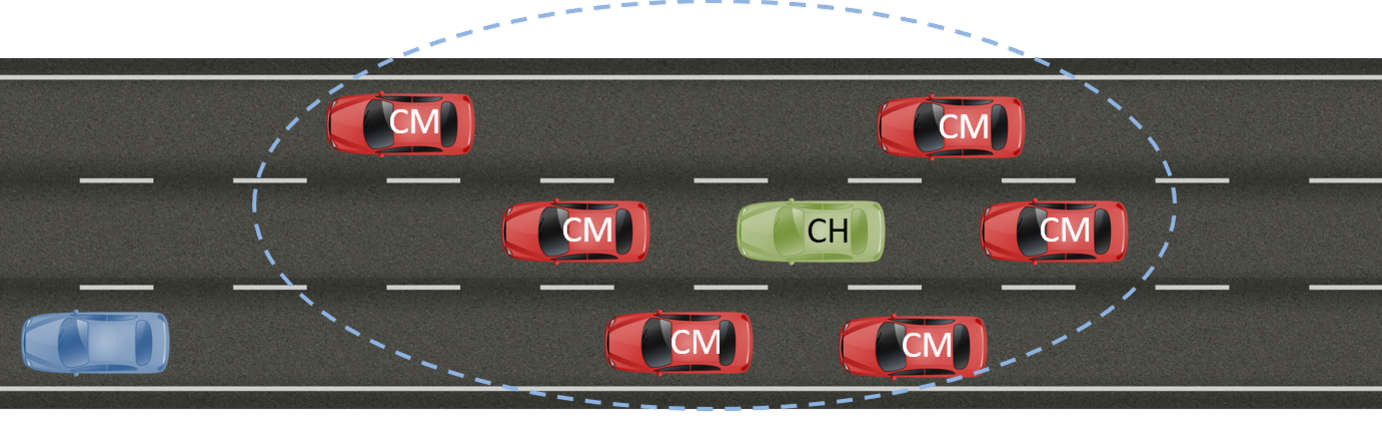
\includegraphics[width=0.9\textwidth]{figures/cluster}
    \caption{Typical \ac{VANET} cluster }
    \label{fig:cluster}
\end{figure}

\chapter{Clustering methodologies}
\label{sec:methodologies}

To achieve a robust and effective communication in the high mobility environment, \ac{VANET} applications use various
parameters to cluster the nodes into meaningful sub-groups based on the application requirement. This leads to a wide
range of clustering methodologies which define applications specific algorithms useful for respective application or
a generic algorithm with possibility to handle different requirements. In this chapter, we discuss some of the common
parameters used individually or in combination with each other to define thresholds for vehicles to join cluster and
cluster head selection along with some methodologies which uses them for clustering.

\section{Clustering Parameters}

Parameters play an important role to build stable cluster effectively which can be used to perform the application
specific communication with minimal overhead. Some of the common parameters which are used by the algorithms to
form basis for threshold calculation are summarized in \cref{tab:parameters}.

\begin{longtable}{>{\raggedright}p{3.5cm}p{7.5cm}}
    \hline
    Parameter               & Description                                                                                                          \\
    \hline
    \endhead
    \hline
    \endfoot
    \hline
    \caption{Common clustering parameters}\label{tab:parameters}                                                                                                \\
    \endlastfoot
    Vehicular mobility      & This is the most common parameter used in the algorithms. Mobility of the vehicles are measured in terms of
    relative velocity and average velocity over time of the vehicle                                                                                \\
    Direction of the travel & In many cases, information to be shared between vehicles only has relevance if the vehicles share the same path
    and direction. This knowledge can be used by the algorithms for forming trajectory tables or assigning Road IDs
    to compare directions and route                                                                                                                \\
    Destination             & Used by applications which give importance to route taken by the vehicles to provide longer stable cluster            \\
    Density                 & Mostly used to differentiate sparse and dense networks and define different communication model to ensure reliable
    communication in both scenarios                                                                                                                \\
    Unique ID               & Simplest clustering parameter, commonly used to identify and cluster vehicles requiring multi-hop reliable communication \\
    Location                & Used with application requiring location based information such as intersection support and congestion avoidance     \\
\end{longtable}

\section{Typical clustering Operations}

To group vehicles together, there are two main set of operations used by the clustering algorithms. First are the cluster creation operations
as shown in \cref{fig:creation}.

\begin{figure}
    \centering
    \subfloat[Cluster creation with single vehicle]{\label{fig:operation1}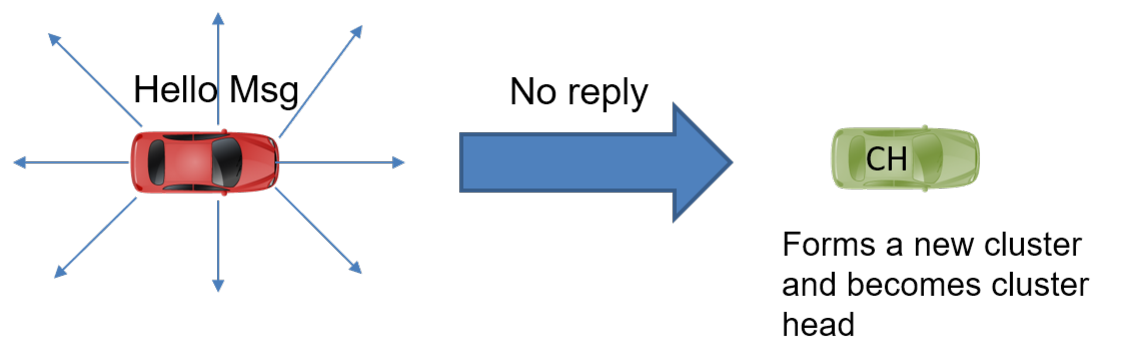
\includegraphics[width=0.9\textwidth]{figures/cluster-step1}}%
    \vfill%
    \subfloat[Cluster creation with multiple vehicles]{\label{fig:operation2}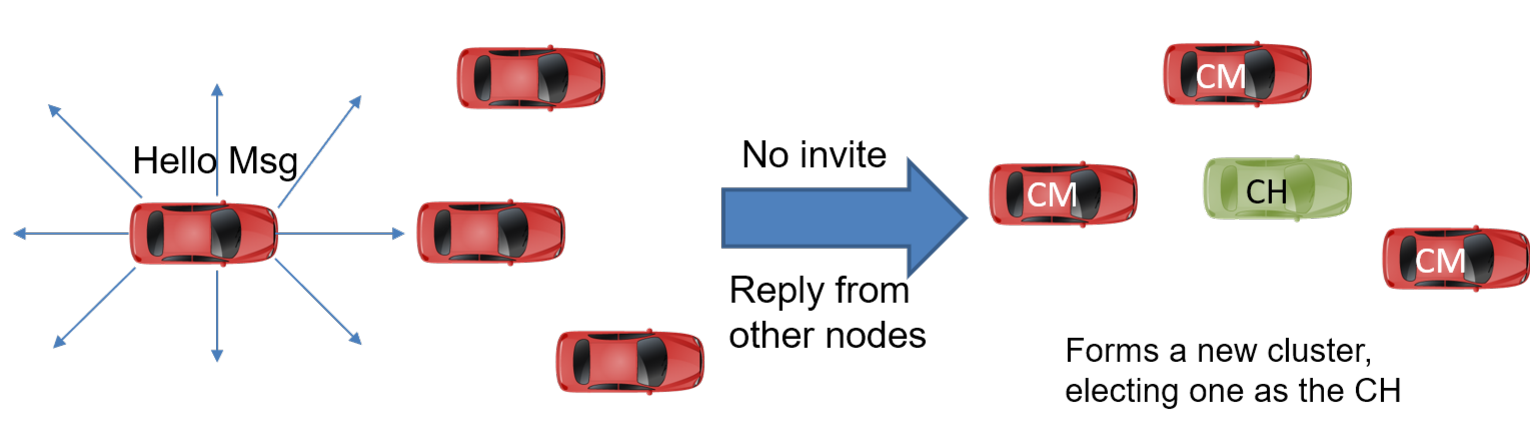
\includegraphics[width=0.9\textwidth]{figures/cluster-step3}}

    \caption{Cluster creation operations}
    \label{fig:creation}
\end{figure}

As the name suggest these operations are used to create a new cluster after verifying the fitness of the
participants. \cref{fig:operation1} shows a case where there is no vehicle around. The vehicle first sends the \texttt{HELLO} messages to
discover presence of another cluster and after a certain timeout identifies that there is no one around and starts a new cluster, becoming the
new \ac{CH}. The second operation depicted in \cref{fig:operation2} is used when there are vehicles in the vicinity which have not yet formed
any cluster. In this case the vehicles discover each other via \texttt{HELLO} messages and form a cluster followed by an election of the
\ac{CH}.

The second set of operations are used for cluster maintenance shown in \cref{fig:maintenance}. Cluster joining operation shown in \cref{fig:operation3}
is used to add new members to the cluster. The request to join is initiated by the vehicle by sending the \texttt{HELLO} message. When the \ac{CH} receives
this message, it verifies if the vehicle is fit to join the cluster and then invites it using \texttt{INVITE} message. Cluster merging happens when two
\ac{CH} come in contact with each other as shown in \cref{fig:operation4}. At this point the \ac{CH}s decide to merge the clusters if the current state of
the two cluster is similar in terms of the cluster parameters. After merging, one of the existing \ac{CH} becomes the new \ac{CH} of the merged cluster and
the other \ac{CH} becomes a \ac{CM}.

It should be noted that the actual implementation of these operations may change from one methodology to another depending upon the parameter and the
use case for the clustering.

\begin{figure}
    \centering
    \subfloat[Cluster joining]{\label{fig:operation3}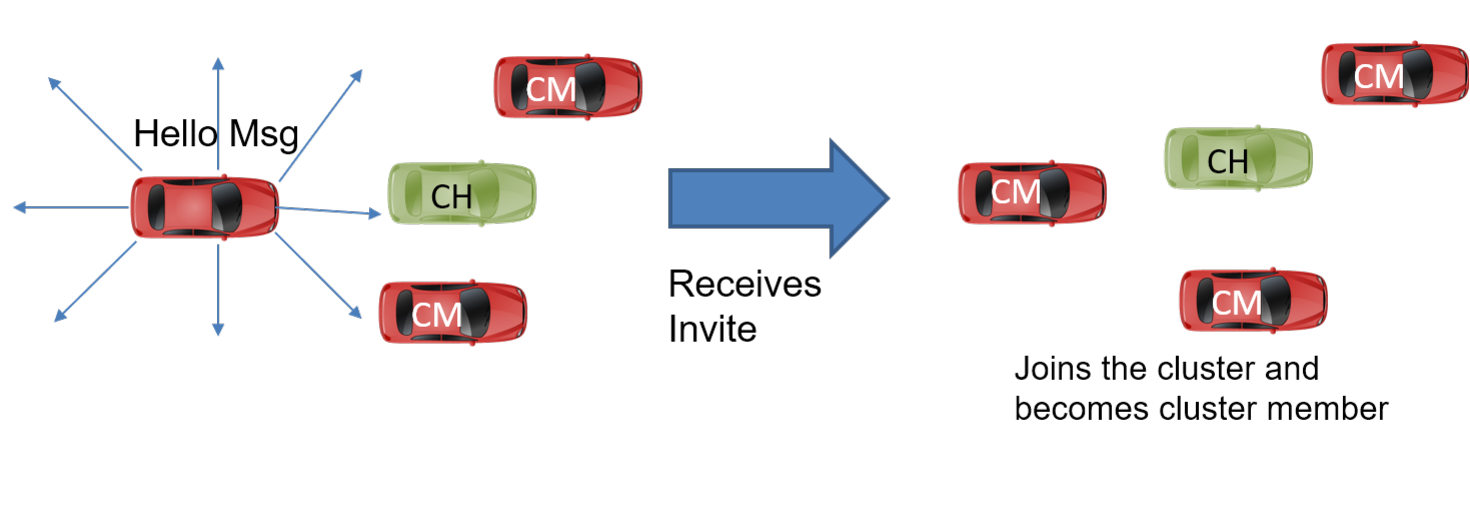
\includegraphics[width=0.9\textwidth]{figures/cluster-step2}}%
    \vfill%
    \subfloat[Cluster merging]{\label{fig:operation4}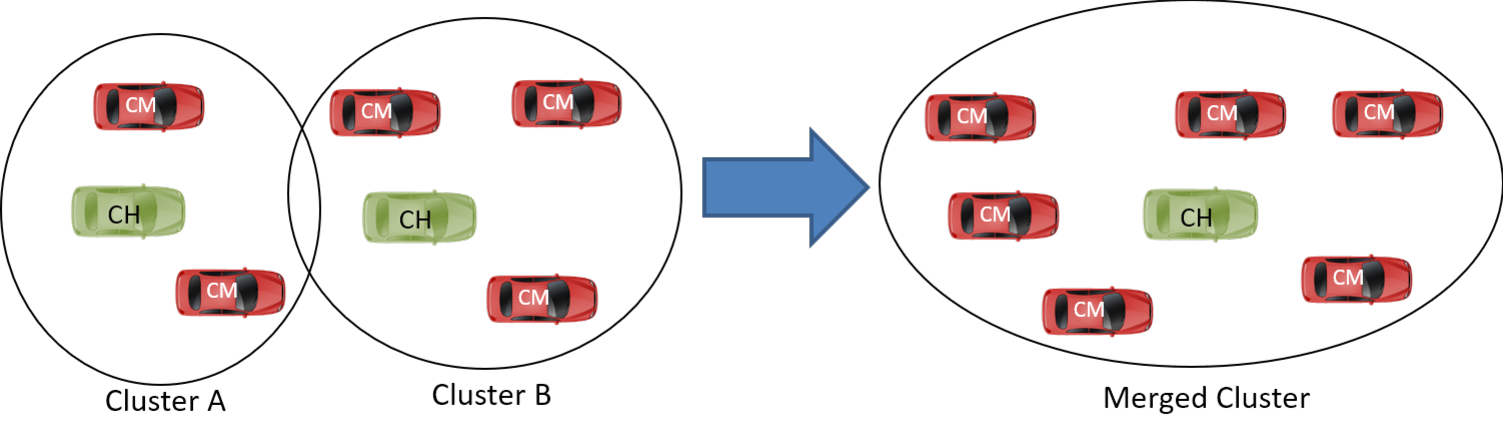
\includegraphics[width=0.9\textwidth]{figures/cluster-step4}}

    \caption{Cluster maintenance operations}
    \label{fig:maintenance}
\end{figure}

\section{Methodologies}

This section presents some of the methodologies which are popular and used as the basis for several algorithms designed for clustering
in \ac{VANET}.

\subsection{Clustering using vehicular mobility}

Vehicular mobility is one of the common and vastly used methodology for clustering. Relative velocity which can be used to differentiate
the vehicles into different sub-groups is used as one of the main parameters in such algorithms. The vehicle mobility is the main element
affecting the network topology which the algorithms use to estimate dynamicity of the network and improve stability. Clustering algorithms
presented by \textcite{ARKIAN2014197, 6737622, 6077004} use relative velocity as the main parameter to define the cluster joining and cluster
head selection metrics.

\subsection{Clustering using direction and destination}

It has been identified that vehicles which travel in same direction or to same destination are supposed to be benefited
most if they share information to each other. This makes the direction of travel and destination based clustering other
important parameters used for clustering. This methodology requires the vehicles to be equipped with \ac{GPS} devices to
get accurate location information. There can be variations based on the calculation and comparison of the routes of the
vehicles. The methodology presented by \textcite{6685518} uses trajectory tables to store position information which is
then shared and compared by the vehicles to check the direction and route of travel whereas methodology presented
by \textcite{5416361} calculates the direction at intersection points based on the turn the vehicles are going to take.
\textcite{5735785} has proposed a method which uses lane based information to decide the direction and cluster the vehicles.

\subsection{Clustering using vehicular density}

Density of the vehicles varies based on the environment considered. This is often utilized by the clustering
algorithm as an important parameter to define different communication methodologies for dense network in city vs
sparse network on highways. Aim of such algorithms is to reduce network congestion in cities by avoiding unnecessary
flooding and provide longer network coverage on highways using long range communication. \textcite{4976256} discusses
one such algorithm which uses density based clustering to define different communication model based on connectivity and
link quality estimates.

\subsection{Hybrid clustering}

Some application may require use of more than one parameter to make decision. Clustering algorithms defined for such
application are complex and use multiple parameters in combination to each other. The clustering scheme proposed
in \cite{6077004} uses a combination of location, vehicular velocity and destination information to build up clusters
which can adapt with changes in any of the parameters. Such methods are always complex and require a lot of communication
between the vehicles to share real-time information.

\subsection{Multi-hop clustering}

The methodologies summarized till now, relies on one hop communication i.e. direct communication between
the \ac{CH} and the \ac{CM}. The one hop based communication clusters face the problem of frequent handoffs between
the clusters for members with high mobility. Multi-hop clustering methods try to address this issue by including N-hop
members to the cluster. As shown in \cref{fig:2hop} and \cref{fig:3hop}, the multi-hop members communicate to the \ac{CH}
via the intermediate members and can be located a maximum of N-hop distance away from the \ac{CH}. In a multi-hop
clustering methodology, the \texttt{HELLO} messages contain additionally the number of current hops and are re-broadcasted
by a node after adding themselves as an intermediate node. This forms the basis for identifying routes to the N-hop nodes
after clustering. \textcite{Zhang2069135} and \textcite{6554933} present clustering methods based on multi-hop schemes
along with vehicular mobility.


\begin{figure}[h]%
    \centering
    \subfloat[1 Hop]{\label{fig:1hop}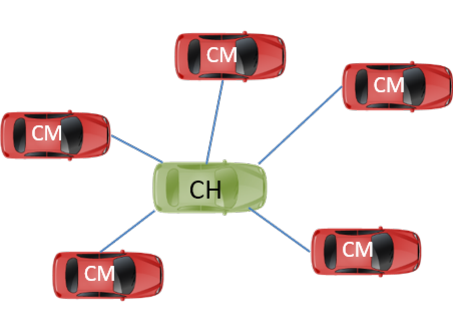
\includegraphics[width=0.3\textwidth]{figures/1hop}}%
    \hfill%
    \subfloat[2 Hop]{\label{fig:2hop}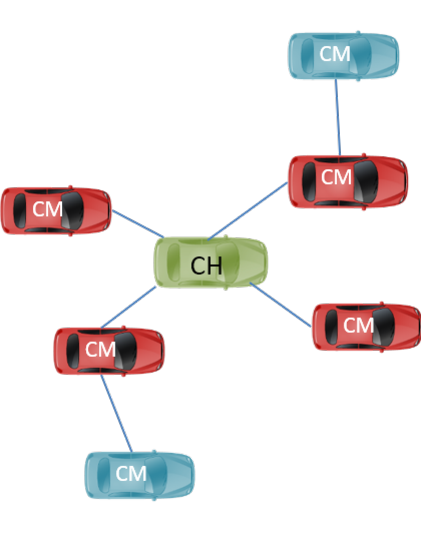
\includegraphics[width=0.3\textwidth]{figures/2hop}}%
    \hfill%
    \subfloat[3 Hop]{\label{fig:3hop}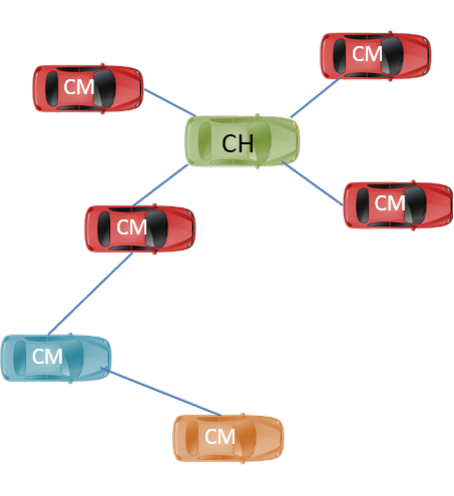
\includegraphics[width=0.3\textwidth]{figures/3hop}}
    \caption{Multi-hop clustering (based on~\cite[Figure~1]{6554933})}%
    \label{fig:multihop}%
\end{figure}


\chapter{Evaluation and analysis techniques}
\label{sec:evaluation}

Implementing a proposed solution for \ac{VANET} with real vehicles for testing is not straight forward.
It always requires availability of various equipment and testing environment to implement a prototype system which
would be suitable for evaluating the proposed method. Due to this, most of the authors of the proposed solution use
simulation as the main method of evaluation and producing data for evaluation. This chapter will discuss some of
the important tools and techniques used for evaluation of clustering methodologies for \ac{VANET} and present
the common metrics derived from the simulation data for comparison.

Simulation for \ac{VANET} involves two aspects, first is modelling the vehicular mobility and second is modelling the
network communication between the vehicles. Another major challenge is to define the interlink between these models
to build a realistic simulation environment. Some of the popular network simulators used are OMNET++\footnote{\url{https://www.omnetpp.org/}},
ns3\footnote{\url{https://www.nsnam.org/}} and VanetMobiSim~\cite{4127230}. Vehicular mobility can be defined by SUMO~\cite{dlr71460}
which is most popular tool capable of managing vehicular mobility via predefined traffic scenarios or some specific mobility model.
\textcite{sommer2011bidirectionally} presented \ac{VEINS} which defines extensions to interconnect OMNET++ and SUMO. A combination of
these tools is used to provide simulation environments for evaluating the clustering methodologies.

\section{Important parameters for evaluation}

Choosing correct simulation parameters is important for producing data which is suitable to derive metrics for evaluation.
It mostly depends on the characteristics of the simulated model which in this case is clustering methods so mostly depends
on the parameters~\cref{tab:parameters} chosen for clustering and some typical networking and vehicular mobility
characteristics. \cref{tab:simparams} lists down some of the parameters along with their typical values in simulation environment.

\begin{table}[h]
    \centering
    \begin{tabular}{>{\raggedright}p{5.4cm}p{3.4cm}}
        \toprule
        Parameter                 & values                                                                                                                         \\
        \midrule
        Simulation Time           & \SI{120}{\second} - \SI{400}{\second}                                                                                          \\
        Route length              & \SI{3}{\kilo\meter} - \SI{10}{\kilo\meter}                                                                                     \\
        Average speed of Vehicles & \SI{10}{\meter\per\second} - \SI{40}{\meter\per\second}                                                                        \\
        Transmission rate         & \SI[per-mode=symbol,per-symbol = p]{6}{\mega\bits\per\second} - \SI[per-mode=symbol,per-symbol = p]{27}{\mega\bits\per\second} \\
        Communication range       & \SI{100}{\meter} - \SI{400}{\meter}                                                                                            \\
        Size of messages          & \SI{100}{\byte} - \SI{150}{\byte}                                                                                              \\
        No. of vehicles/Flow rate & \SI{1800}{\vehicle\per\hour} - \SI{3600}{\vehicle\per\hour}                                                                    \\
        \bottomrule
    \end{tabular}
    \caption{Typical simulation parameters}
    \label{tab:simparams}
\end{table}

\section{Analysis of results}

Once the data is captured using the simulation of the target clustering methods, it should be used for analysis against some
metrics which allows comparative evaluation of the proposed schemes. Some of the important metrics which are used to compare
the performance of the clustering algorithms for \ac{VANET} are as follows.

\begin{itemize}
    \item \textbf{Cluster head duration/Cluster lifetime}: Most important metrics used to measure the stability of clusters.
          Longer duration of \ac{CH} is resultant of stable clusters which can perform better in a dynamic environment.
    \item \textbf{Number of clusters}: This metric gives quality of formation of the clusters. Higher number of clusters
          would lead to cluster merging and increased cluster formation overhead whereas smaller number means large cluster sizes
          which would result in cluster division due communication failures in high mobile environment.
    \item \textbf{Cluster member duration/Connectivity}: Longer member duration are important for stability and effective
          communication. Member duration is also a measure of connectivity and the link quality achieved by the clustering method
          which directly affects the network communication between the nodes.
\end{itemize}


\chapter{Conclusion}
\label{sec:conclusions}

This thesis introduces the reader with the requirements for clustering in vehicular networks along with various
terminologies and methodologies proposed in literature by various researchers. It also gives a brief overview
of tools and metrics which are important for the evaluation of methodologies in \ac{VANET} systems. The methodologies
mentioned in this thesis only provides a brief introduction to the main ideas for clustering in vehicular networks to
the reader.

Currently, there is a huge advancement being made in the wireless communication technologies which will open
various new opportunities for improving the communication environment for \ac{VANET}s in the future.
Improved communication mechanisms for \ac{V2V} and \ac{V2I} communication would provide more stable and
reliable communication channels. Thus, providing basis for improving existing clustering methodologies by
extending them to use new technology and design new methodologies to achieve better performance in terms
of stability and networking connectivity.

I believe this thesis should be a good starting point for introducing the concept of clustering in vehicular
network and highlighting the major areas which the reader can further explore based on their needs.

\cleardoublepage

\listofabbreviations
\clearpage

\listoffigures
\clearpage

\listoftables
\clearpage

\printbibliography

\end{document}
